\subsection*{Partie I. Polynômes de Bernoulli}
Dans toute la correction, on identifie un polynôme avec la fonction associée et on se passe donc des tildes. En revanche, on note $\widehat{P}(Q)$, le polynôme obtenu à partir de $P$ en substituant $Q$ à $X$.
\begin{enumerate}
  \item Les polynômes $P_n = X^n$ satisfont aux conditions. Cette question ne figure que pour introduire une certaine analogie avec les polynômes de Bernoulli. 

 \item Tout polynôme admet des polynômes primitifs (c'est à dire dont la dérivée est égale au polynôme donné). Deux de ces polynômes primitifes ne diffèrent que d'une constante que l'on peut ajuster pour assure la nullité de l'intégrale.
 Par exemple 
\begin{displaymath}
B_1'=1\,B_0 \Rightarrow B_1 = X + \lambda \text{ avec } \int_0^1B(t)\,dt = \frac{1}{2}+\lambda
\end{displaymath}
L'unique possibilité est donc 
\begin{displaymath}
  B_1 = X -\frac{1}{2}
\end{displaymath}
Pour un entier $n$ fixé et des polynômes $B_0,\cdots, B_n$ vérifiant les conditions, il existe un unique polynôme $B_{n+1}$ vérifiant les conditions. Il est obtenu en calculant la constante d'intégration qui assure la nullité de l'intégrale. On trouve en particulier
\begin{displaymath}
B_2 = X^2 - X + \frac{1}{6},\hspace{0.5cm}
B_3 = X^3 - \frac{3}{2}X^2 + \frac{1}{2}X = X(X-1)(X-\frac{1}{2})
\end{displaymath}
On montre par récurrence que $B_n$ est unitaire (coefficient dominant 1) de degré $n$.
 
 \item
\begin{enumerate}
 \item Pour $n\geq 2$, les valeurs en $0$ et $1$ sont égales car
\begin{displaymath}
 B_{n}(1)-B_{n}(0) = \int_0^1B_{n}'(t)\,dt = n \int_0^1B_{n-1}(t)\,dt = 0
\end{displaymath}
par définition. La valeur commune est notée $\beta_n$. On a déjà calculé
\begin{displaymath}
  \beta_1 = -\frac{1}{2},\hspace{0.5cm} \beta_2 = \frac{1}{6},\hspace{0.5cm}  \beta_3 = 0
\end{displaymath}

 \item \label{sym} Introduisons des polynômes $C_n$ par: 
\begin{displaymath}
  C_n = (-1)^n\widehat{B_n}(1-X)
\end{displaymath}
On va montrer que la suite des $C_n$ vérifie \emph{les mêmes relations} que la suite des $B_n$. Ces relations définissant une \emph{unique} suite de polynômes, cela assure que $C_n=B_n$ pour tous les $n$.
\begin{displaymath}
 B_0=1 \Rightarrow C_0=1
\end{displaymath}
\begin{displaymath}
 C_{n+1}'(x) = -(-1)^{n+1}B_{n+}'(1-x)=(-1)^nB_n(1-x)=C_n(x)
\end{displaymath}
Pour la relation intégrale, on utilise le changement de variable $u=1-x$:
\begin{displaymath}
 \int_0^1C_n(x)\,dx = -\int_1^0C_n(1-u)\,du = (-1)^n \int_0^1B_n(u)\,du =0
\end{displaymath}

 \item D'après la question précédente, pour tout $n$ impair, on a $B_n(\frac{1}{2}) = - B_n(\frac{1}{2})$ donc $B_n(\frac{1}{2})$ est nul. C'est vrai aussi pour $n=1$ d'après l'expression de $B_1$.\newline
Toujours pour $n$ impair, on a aussi $B_n(1) = -B_n(0)$ qui se combine avec $B_n(1)=B_n(0)$ ($n\geq 2$ seulement) pour donner $B_n(1)=B_n(0)=0$.\newline
En conclusion, $\beta_n = B_n(1) = B_n(0)$ et $B_n(\frac{1}{2})$ sont nuls pour tous les entiers impairs supérieurs ou égaux à $3$.
\end{enumerate}

 \item On veut démontrer par récurrence que les $B_n$ avec $n$ impair supérieur ou égal à $3$ ne s'annulent pas dans $]0,\frac{1}{2}[$. \`A cause des propriétés déjà montrées cela siginifie que $0$, $\frac{1}{2}$, $1$ sont les seules racines.\newline
La récurrence est initialisée à $3$ grace à la factorisation de $B_3$.\newline
On raisonne par l'absurde avec le théorème de Rolle.\newline
Supposons que $B_{2m+1}$ s'annule en $c$ avec $0<c<\frac{1}{2}$. En appliquant le théorème de Rolle à $B_{2m+1}$ entre $0$ et $c$ puis entre $c$ et $\frac{1}{2}$, on prouve l'existence de racines $d$ et $d'$ de $B_{2m}$ telles que $0<d<c<d'<\frac{1}{2}$. On peut alors appliquer le théorème de Rolle à $B_{2m}$ entre $d$ et $d'$. Cela entraine l'existence d'une racine $u$ de $B_{2m-1}$ entre $d$ et $d'$ donc telle que $0<u<\frac{1}{2}$.

On peut aussi raisonner directement avec la convexité. Dans l'intervalle $[0,\frac{1}{2}]$, la fonction $B_{2n-1}$ garde un signe constant et c'est la dérivée seconde de $B_{2n+1}$. On en déduit que $B_{2n+1}$ est soit concave soit convexe. Son graphe est donc toujours au dessus ou au dessous de ses cordes. La corde entre les points d'abscisses $0$ et $\frac{1}{2}$ est un segment de l'axe car la fonction s'annule en ces points. On en déduit facilement de plus que les signes s'alternent d'un entier impair au suivant.\newline 
Montrons maintenant que $B_m - \beta_m$ garde un signe constant sur $[0,1]$ c'est à dire que $0$ et $1$ sont des extréma globaux de $B_m$ sur $[0,1]$.\newline
D'après le théorème des valeurs intermédiaires, $B_{2m}(x)-B_{2m}(0)$ est du signe de $B_{2m-1}$ pour $m\geq2$ et $0<x<\frac{1}{2}$. Par symétrie (question \ref{sym}), on peut écrire
\begin{multline*}
\forall x >\frac{1}{2}, \; B_{2m}(x)-B_{2m}(0)=B_{2m}(x)-B_{2m}(1) + \underset{=0}{\underbrace{B_{2m}(1) - B_{2m}(0)}} \\
= B_{2m}(1-x)-B_{2m}(0)
\end{multline*}
donc le signe est le même que dans la première moitié de l'intervalle.
\begin{figure}[h]
  \centering
  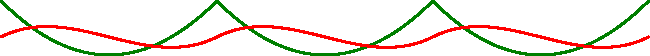
\includegraphics{./Cbernsomm_1.pdf}
  % Cbernsom_1.pdf: 0x0 pixel, -2147483648dpi, 0.00x0.00 cm, bb=
  \caption{graphes de $b_2$ et $b_3$}
  \label{fig:Cbernsomm_1}
\end{figure}

\item Les fonctions de Bernoulli $b_n$ sont définies par $b_n(x) = B_n(\left\lbrace x\right\rbrace )$. Elles sont donc périodiques de période $1$ par définition.
\begin{enumerate}
  \item Dans un intervalle $]p,p+1[$ ouvert entre deux entiers, $b_n(x)= B_n(x-p)$, elle est donc de classe $\mathcal{C}^{\infty}$ comme la fonction polynomiale $B_n$. De plus
\begin{displaymath}
  b_n'(x) = B_n'(x-p) = nB_{n-1}(x-p) = nb_{n-1}(x)
\end{displaymath}

  \item La restriction de $b_1$ à un segment est intégrable car elle est continue par morceaux, les entiers de ce segment constituant une subdivision adaptée.
  
  \item Pour $n\geq 2$, les valeurs de $B_n(0)$ et de $B_n(1)$ sont égales, les fonctions $b_n$ sont donc continues (en particulier $b_2$). Les relations de la question a. s'étendent par continuité aux points entiers :
\begin{displaymath}
  b_2 \in \mathcal{C}^0 \Rightarrow b_3\in \mathcal{C}^1 \Rightarrow b_4\in \mathcal{C}^2 \Rightarrow \cdots \Rightarrow b_n\in \mathcal{C}^{n-2}
\end{displaymath}
\end{enumerate}

\end{enumerate}

\subsection*{Partie II. Formule sommatoire d'Euler - Mac Laurin}
\begin{enumerate}
  \item Voir cours. Cette question développe l'analogie (initiée en question 1) entre la formule de Taylor avec reste intégral et la formule sommatoire présentée ici. La formule de Taylor avec reste intégral se démontre avec des intégrations par parties. On cherche donc ici aussi à utiliser des intégrations par parties.

  \item On ne peut pas utiliser directement d'intégration par parties car $b_1$ est seulement intégrable mais non dérivable. On utilise plutôt la relation de Chasles
\begin{multline*}
R_1 = \sum_{k=a}^{b-1}\int_k^{k+1}f'(t)b_1(t)\,dt 
= \sum_{k=a}^{b-1}\int_k^{k+1}f'(t)\left( t-k-\frac{1}{2}\right) \,dt \\
= \sum_{k=a}^{b-1}\left( \left[f(t)t\right]_k^{k+1} -\int_k^{k+1}f(t)\,dt - (k+\frac{1}{2})\left[f(t)\right]_k^{k+1}  \right) \\
= \sum_{k=a}^{b-1}\left(\frac{1}{2}f(k+1) + \frac{1}{2}f(k) -\int_k^{k+1}f(t)\,dt \right) \\
= \frac{1}{2}\sum_{k=a}^{b-1}\left(f(k+1) + f(k)\right) - \int_a^{b}f(t)\,dt
\end{multline*}

\item Pour $m\geq 3$, la fonction $b_m$ est au moins $\mathcal{C}^1$ ce qui permet une intégration par parties. Comme $b_m$ prend la valeur $\beta_m$ en n'importe quel entier:
\begin{multline*}
  R_m = \left[ f^{(m-1)}(t)b_m(t)\right]_a^b - \int_a^bf^{(m-1)}(t)mb_{m-1}(t)\,dt\\
  = \beta_m\left( f^{(m-1)}(b)-f^{(m-1)}(a)\right) - mR_{m-1} 
\end{multline*}
On retrouve avec $R_2$ le problème des hypothèses non vérifiées pour l'intégration par parties. On peut contourner le problème en découpant d'abord en intégrales entre $k$ et $k+1$. Sur chaque $]x_k, x_{k+1}[$, on prolonge la restriction de $b_1$ par continuité ce qui permet l'intégration par parties sur chaque segment. En sommant, on obtient la formule demandée.\newline
La formule s'obtient en formant une combinaison linéaire qui élimine les $R_i$:
\begin{align*}
  R_1 &= \frac{1}{2}\sum_{k=a}^{b-1}\left(f(k+1) + f(k)\right) - \int_a^{b}f(t)\,dt & & \\
  R_2 &= \beta_2(f'(b)-f'(a)) - 2 R_1 & &\times (-1)\,\frac{1}{2} \\
  R_3 &= \beta_3(f^{(2)}(b)-f^{(2)}(a)) - 3 R_2 & &\times (+1)\,\frac{1}{3!} \\
  \vdots &                                & & \\
  R_{n} &= \beta_{n}(f^{(n-1)}(b)-f^{(n-1)}(a)) - n R_{n-1} & &\times (-1)^{n-1}\,\frac{1}{n!} \\
  R_{n+1} &= \beta_{n+1}(f^{(n)}(b)-f^{(n)}(a)) - n R_2 & &\times (-1)^{n}\,\frac{1}{(n+1)!}
\end{align*}
En sommant, on obtient 
\begin{displaymath}
\frac{(-1)^{n}}{(n+1)!}R_{n+1} 
= S - \int_a^{b}f(t)\,dt 
+ \sum_{m=1}^{n}\frac{(-1)^m \beta_{m+1}}{(m+1)!}\left( f^{(m)}(b) - f^{(m)}(a)\right) 
\end{displaymath}
Avec
\begin{multline*}
S = \frac{1}{2}\sum_{k=a}^{b-1}\left(f(k+1) + f(k)\right) \\
= \sum_{k=a+1}^{b-1}f(k)+\frac{1}{2}(f(a)+f(b)) 
= \sum_{k=a}^{b}f(k) - \frac{1}{2}(f(a)+f(b))
\end{multline*}
On obtient donc bien la formule annoncée:
\begin{multline*}
\sum_{k=a}^{b}f(k) = \int_a^{b}f(t)\,dt  + \frac{1}{2}(f(a)+f(b)) \\
+ \sum_{m=1}^{n}\frac{(-1)^{m+1} \beta_{m+1}}{(m+1)!}\left( f^{(m)}(b) - f^{(m)}(a)\right) 
+ \frac{(-1)^{n}}{(n+1)!}R_{n+1}
\end{multline*}

 \item 
 Calculons l'intégrale à l'aide d'une intégration par parties. On peut le faire car $n+1\geq3$. Le calcul est analogue aux précédents. Le crochet est nul car $\beta_{n+1} - b_{n+1}$ est nul en $0$ et $1$ et la constante disparait en dérivant. On obtient donc:
\begin{displaymath}
 \int_a^b\left(\beta_{n+1} - b_{n+1}(t) \right)f^{(n+1)}(t)\,dt=
  \int_a^b (n+1)b_{n}(t)f^{(n)}(t)\,dt = (n+1)R_n
\end{displaymath}
Avec la périodicité de $b_{n+1}$, on en déduit 
\begin{multline*}
 |(n+1)R_n|
\leq \int_a^b\left|\beta_{n+1} - b_{n+1}(t)\right|M_{n+1}\,dt \\
\leq \sum_{k=a}^{b-1}\int_k^{k+1}\left|\beta_{n+1} - b_{n+1}(t)\right|M_{n+1}\,dt 
\leq (b-a)\int_0^{1}\left|\beta_{n+1} - b_{n+1}(t)\right|M_{n+1}\,dt
\end{multline*}
Pour $n$ impair, $\beta_{n+1} - b_{n+1}(t)$ est de signe constant et $\int_0^1 b_{2m+2}(t)\,dt=0$ donc
\begin{displaymath}
|(n+1)R_n| \leq (b-a)\left|\int_0^1\left( \beta_{n+1} - B_{n+1}(t)\right) \,dt \right| M_{n+1} 
\leq (b-a)|\beta_{n+1}| M_{n+1}  
\end{displaymath}

 \item Pour $f(t)=t^4$, le reste $R_5$ est nul. La formule sommatoire conduit à
 \begin{displaymath}
\sum_{k=0}^{n}k^4 = \int_{0}^{n}t^4\,dt  + \frac{n^4}{2} + \frac{1}{6}\frac{4n^3}{2} -\frac{1}{30}\frac{4!\, n}{4!}
= \frac{n^5}{5} + \frac{n^4}{2} + \frac{n^3}{3} - \frac{n}{30}
 \end{displaymath}

\end{enumerate}